\setlength{\abovecaptionskip}{0.5pt} 

\section{Numerical stability of Kolmogorov bias potential} \label{sup_sec:bias_z}
        To improve the numerical stability and efficacy of the Kolmogorov bias, it is convenient to reformulate its calculation (Eq.~\ref{eq:kolmogorov_bias}) in terms of the committor-related $z$ collective variable as it allows lifting the numerical problems that may arise from the direct use of $q$ (see Figure~\ref{sup_fig:numerical_issues}).
        Here, we show that this is formally equivalent to expressing as a functional of $q$.
        In the main text, we shown that $q$ is obtained applying a sigmoid-like switching function $\sigma$ to $z$
            \begin{equation}
                q(\textbf{x}) = \sigma(z(\textbf{x}))
                \quad\text{with}\quad
                \sigma(z) = \frac{1}{1+e^{-pz}}
            \end{equation}
        where we set $p=3$.
        Thus, using the chain rule, we can write
            \begin{equation}  
                \frac{\partial{q(\textbf{x})}}{\partial x} = 
                \frac{\partial{\sigma(z)}}{\partial z}\frac{\partial{z}}{\partial x}
            \end{equation} 
        After some elementary algebra, we can equivalently rewrite the bias as
            \begin{equation}  
                V_{K} = \frac{1}{\beta} \big[ \log(|\nabla z|^2) -4\log({1+e^{-pz}} ) -2pz \big] + c
            \end{equation}  
        where $c$ is a constant that thus will not affect free energy calculations.

        Such a bias is equivalent to the original one but has the advantage that $\frac {\partial z}{\partial x}$ has a much higher numerical resolution in the metastable basins, where $q\sim0$ and $q\sim1$.

\begin{figure}[h!]
    \centering
    \begin{minipage}{0.48\linewidth}
        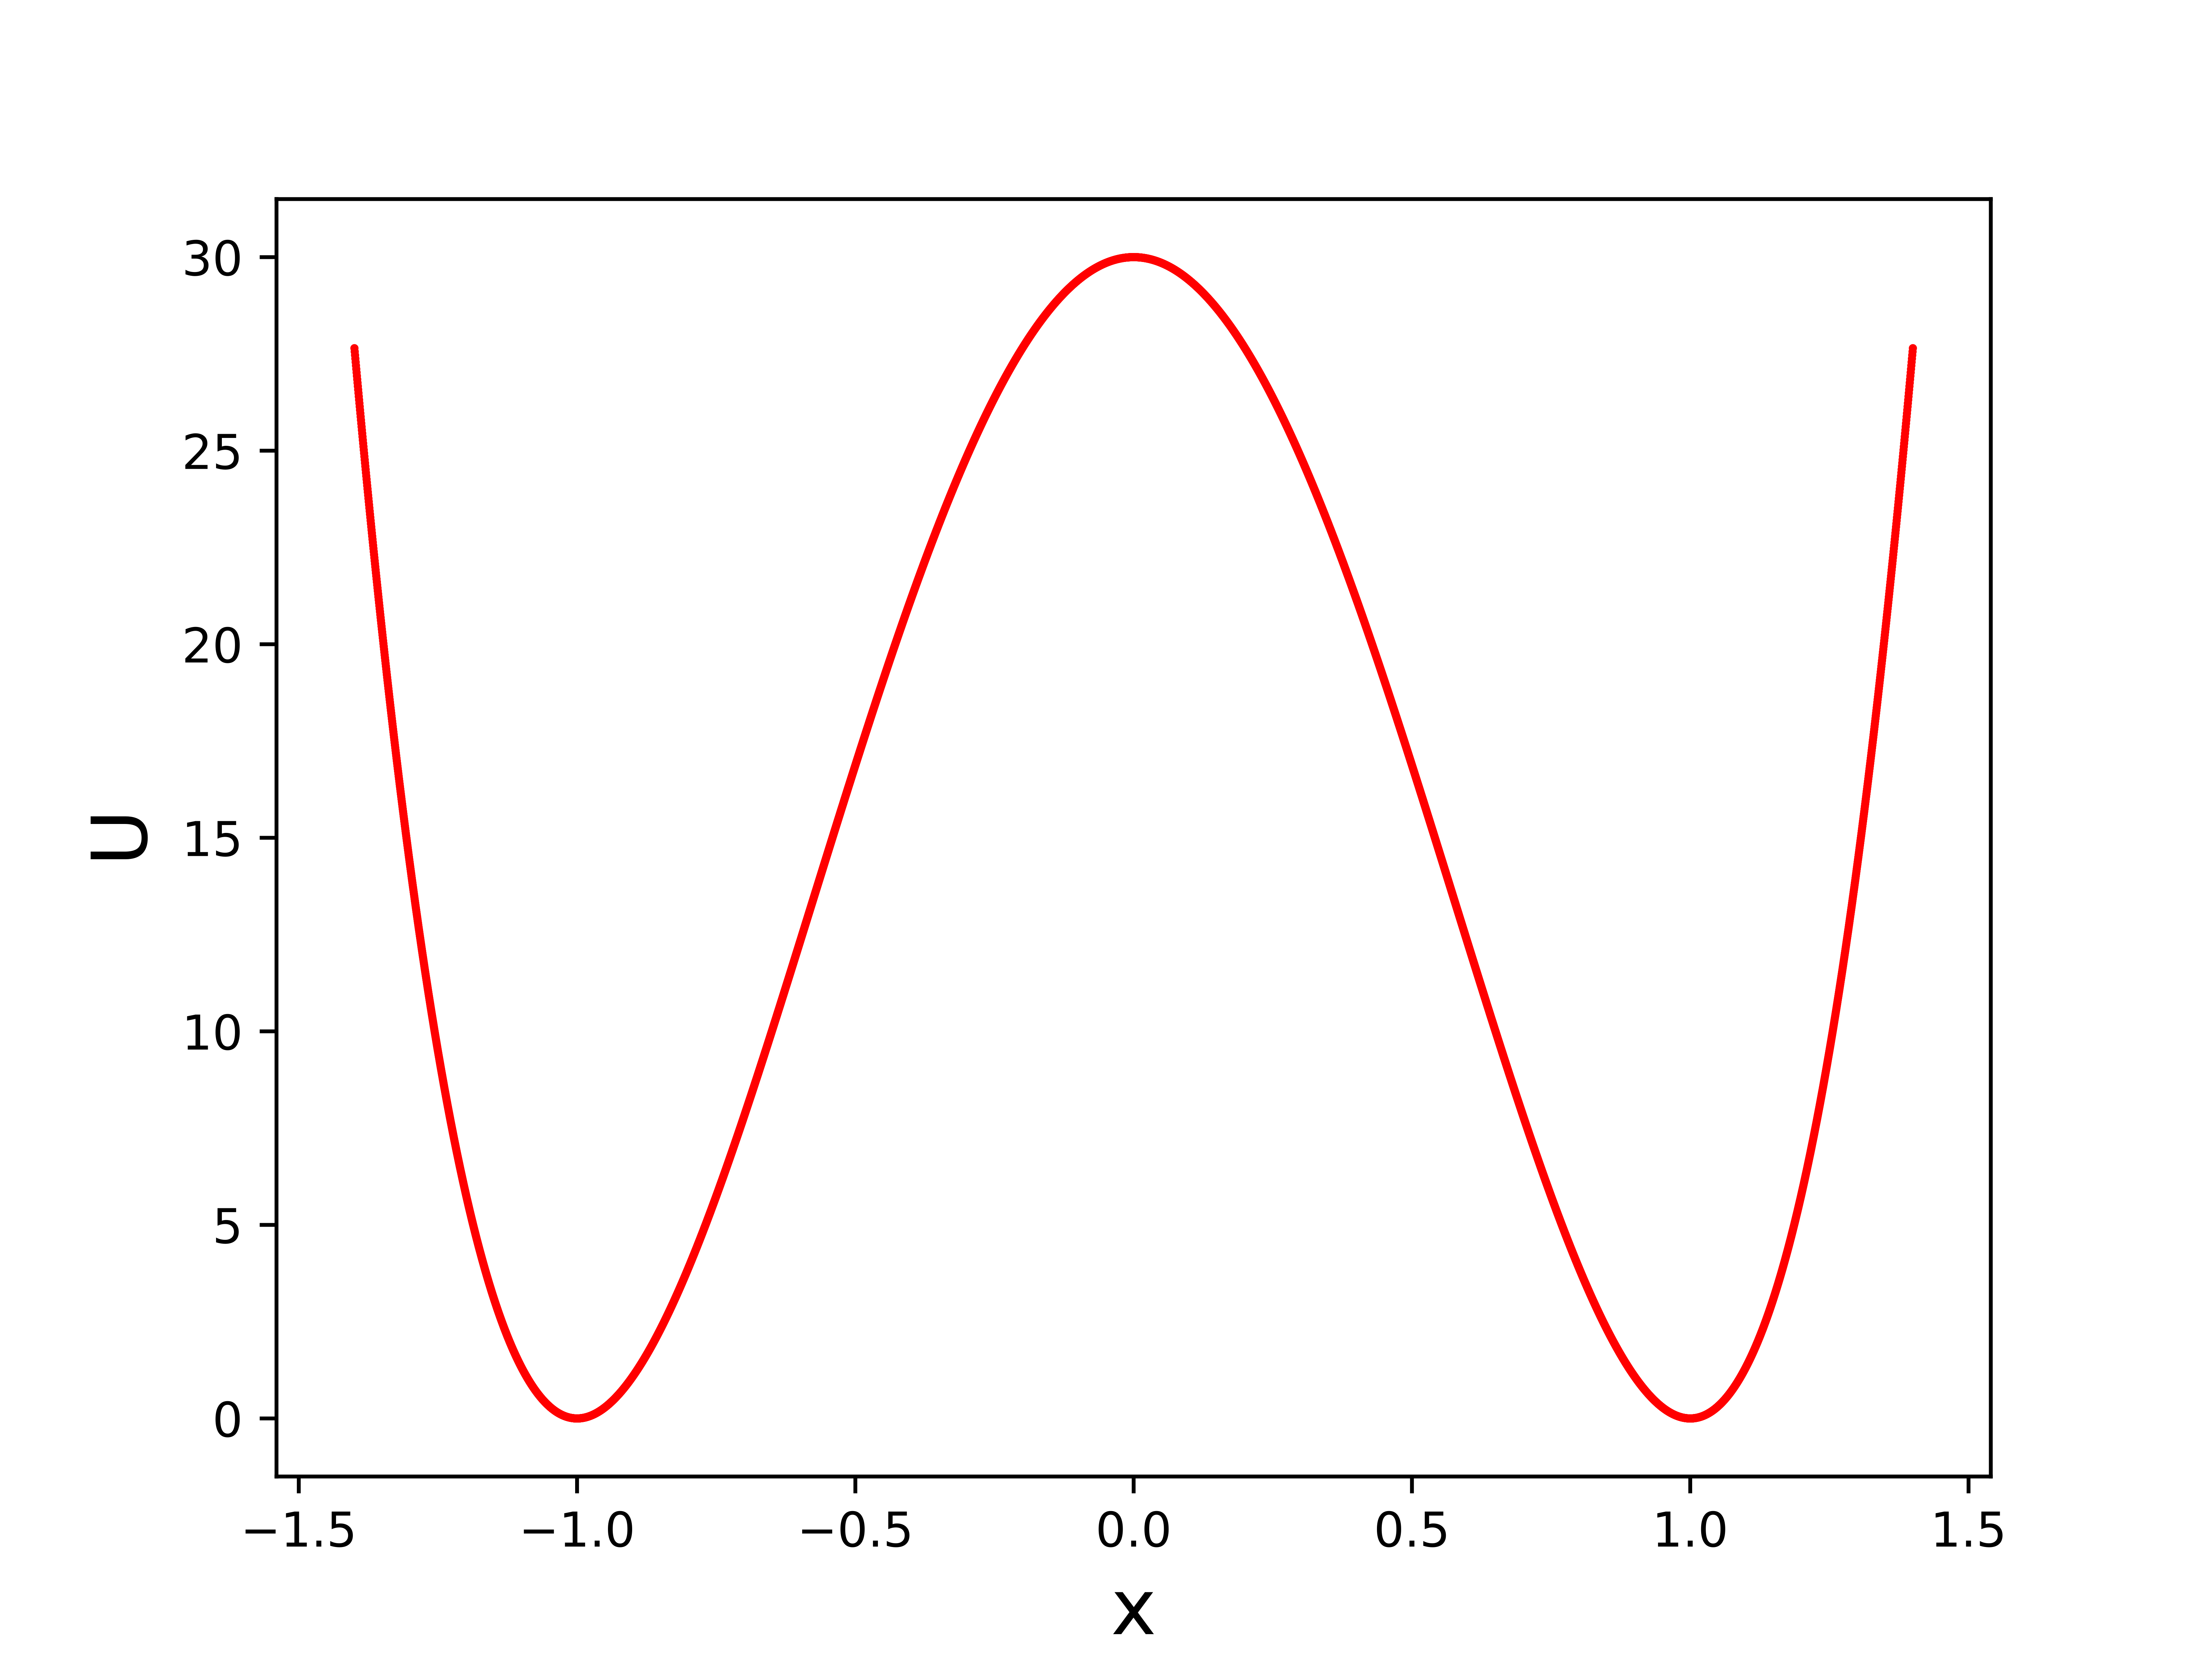
\includegraphics[width=0.8\linewidth]{Figures/SI/double_well_toy.png}
    \end{minipage}
    \begin{minipage}{0.48\linewidth}
        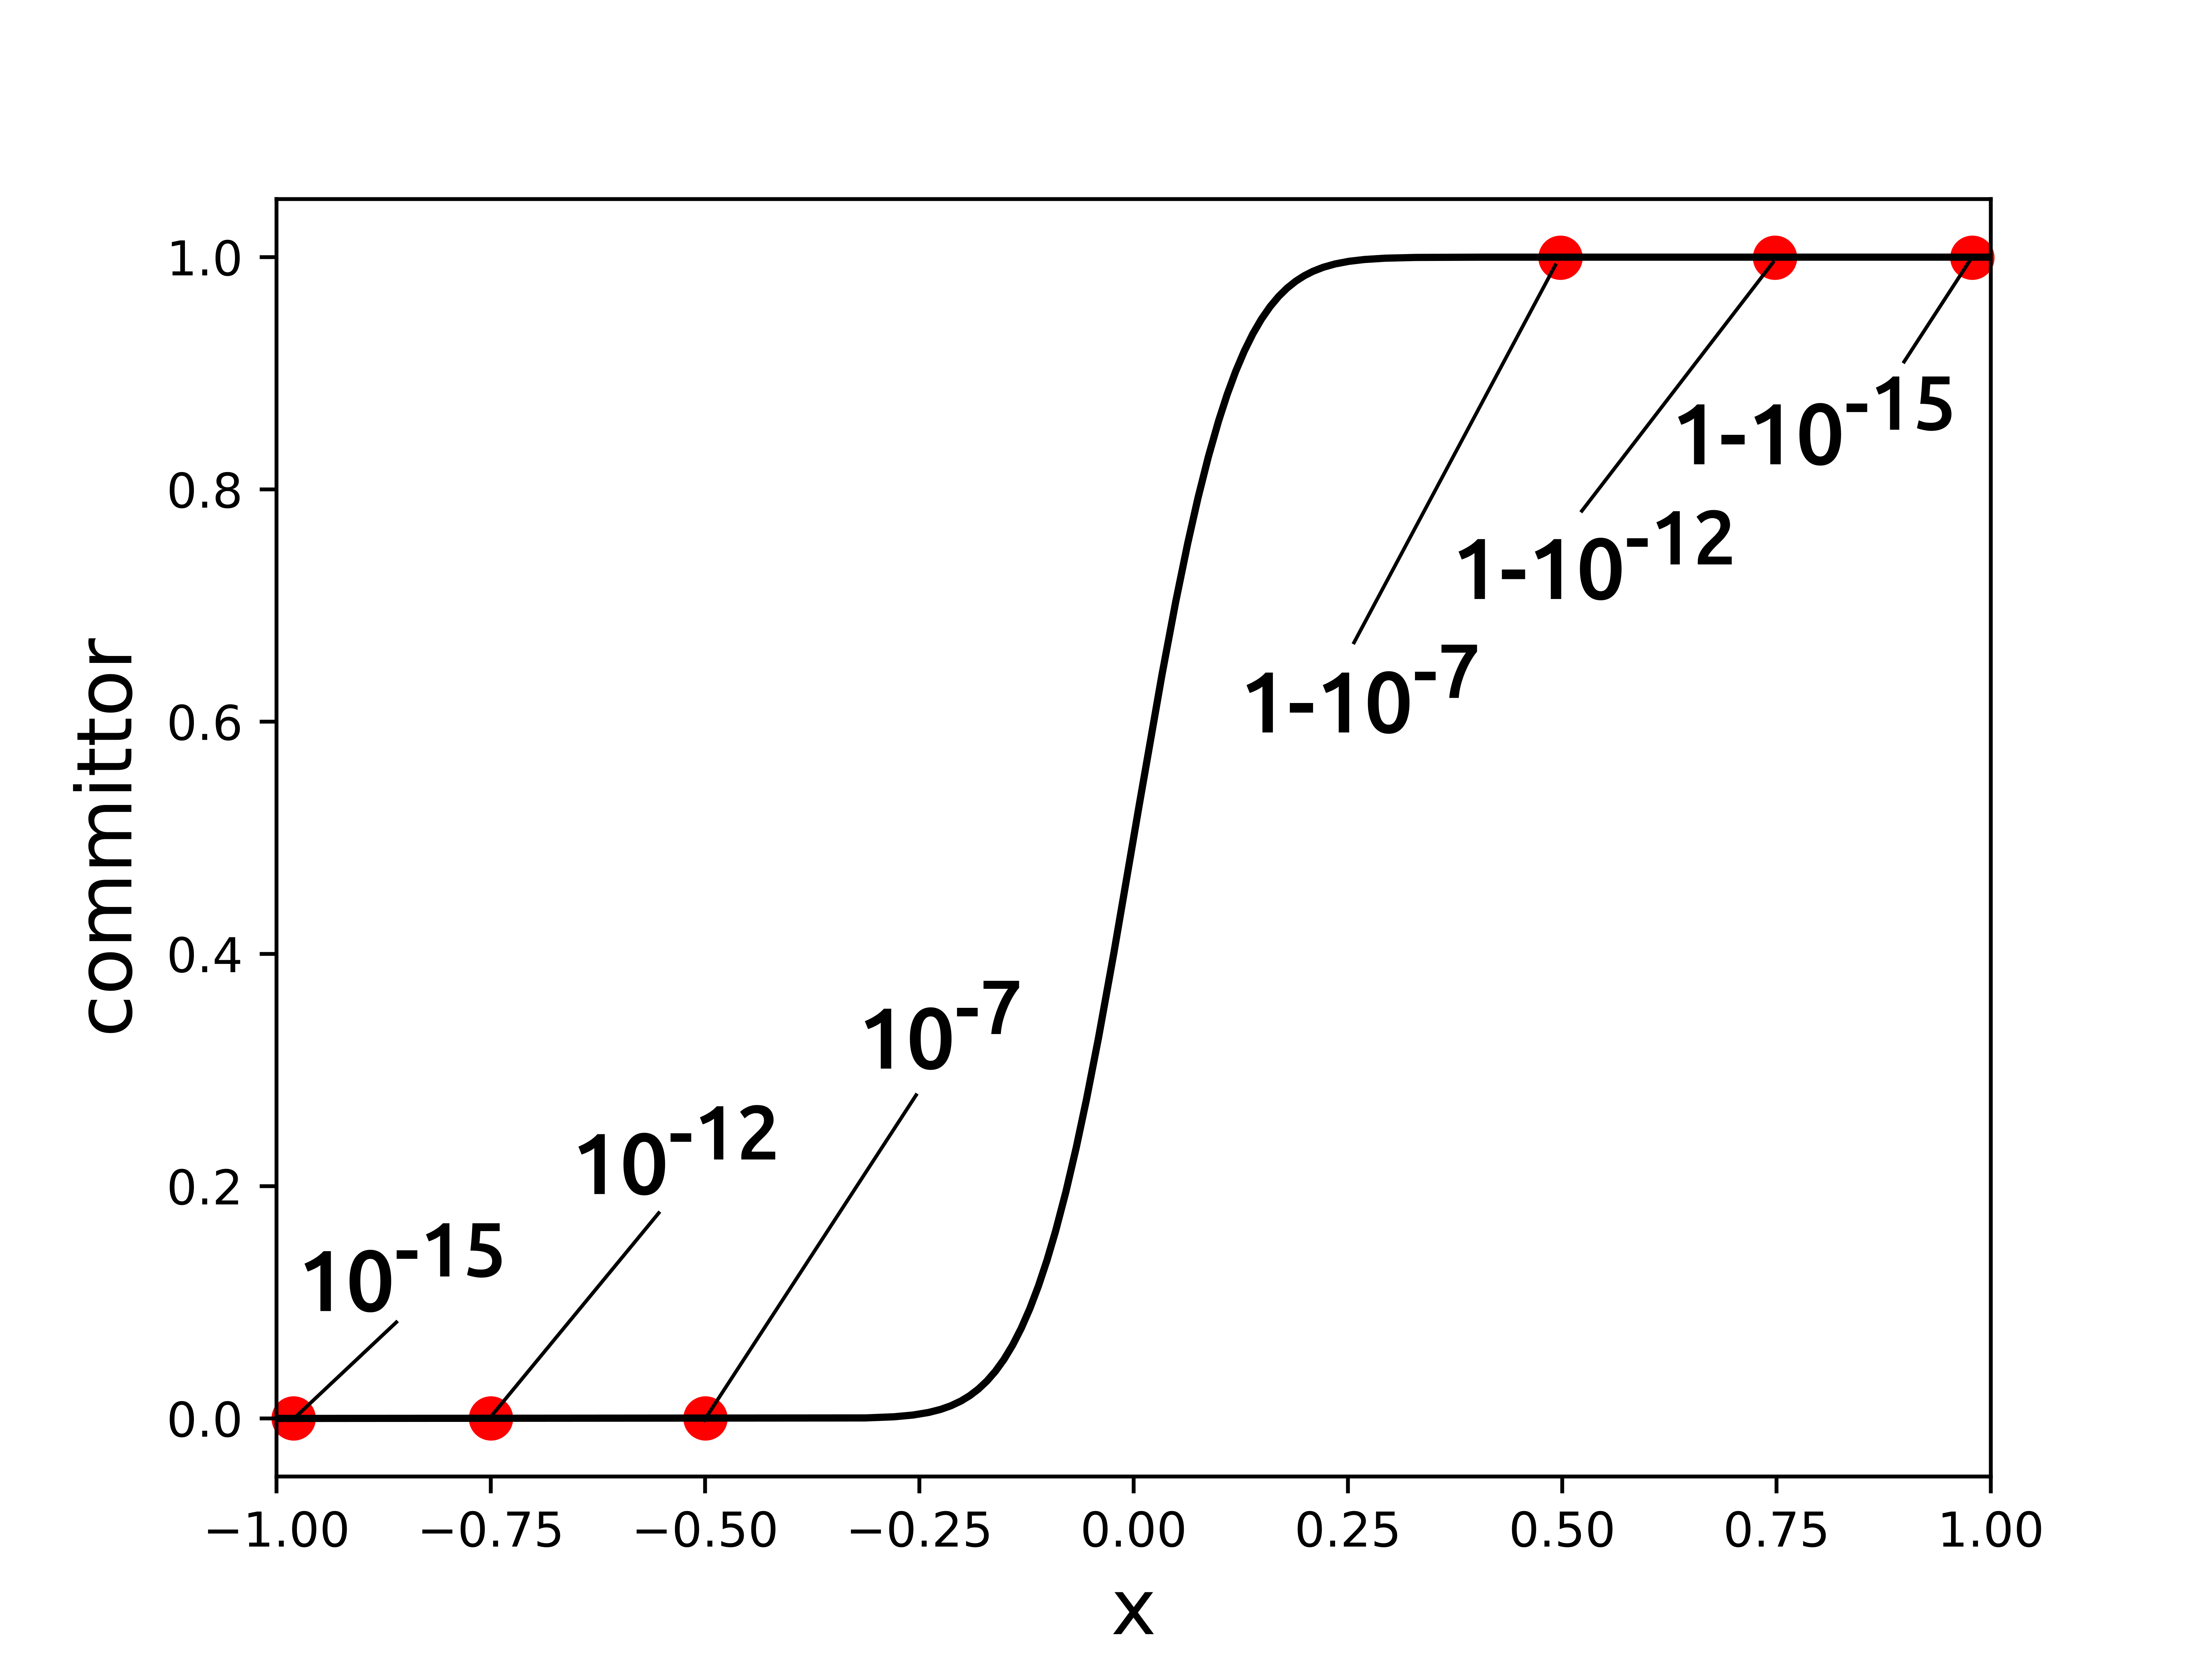
\includegraphics[width=0.8\linewidth]{Figures/SI/committor_numerical.png}
    \end{minipage}
    \caption{\textbf{Numerical issues of the committor function} Visualization of the numerical issue related to the committor function on a toy double-well potential along one dimension x for which an analytical solution can be obtained.}
    \label{sup_fig:numerical_issues}
\end{figure}

% \section{Visualization of the combined bias potential} \label{sup_sec:bias_probability}
%     In Figure~\ref{sup_fig:bias_and_probabilities}, we schematically compare different scenarios both from the energy perspective and the corresponding probability distribution using the simple example of a double-well potential.
    
%     In the unbiased case, the barrier between the two metastable states, A and B, is high enough to make the transition between them a rare event, which is characterized by a negligible probability of sampling the transition state region.
    
%     When the OPES bias is applied to the system, it partially fills the metastable basins, thus lowering the relative height of the barrier, as in other Metadynamics-like enhanced sampling protocols.
%     This favors transitions between A and B passing through the TS, whose probability is enhanced with respect to the unbiased scenario.
%     Nonetheless, the TS is still found at a local maximum of the biased energetic landscape and it is still unfavored with respect to the metastable states.

%     Under the action of the Kolmogorov bias $V_K$, the TS is greatly stabilized, and its probability is greatly enhanced.
%     However, this stabilization is so large and localized that most of the time is spent in the TS and very little in the metastable states.
%     Thus, \emph{full} transitions are hardly observed.

%     If the OPES and Kolmogorov biases are combined, the simulations benefit from both of them.
%     Indeed, the otherwise elusive TS is stabilized by $V_K$, whereas OPES helps in smoothing the energetic landscape and smearing out barriers thus promoting transitions.
%     This way, the probability distribution is spread over the whole relevant phase space, with a greater focus on the metastable states as well as the transition one.
    
% \begin{figure}[h!]
%     \centering
%     \includegraphics[width=0.8\linewidth]{Figures/SI/energy_and_probabilities.png}
%     \caption{Schematic representation of different scenarios from the energy and probability points of view (left and right columns, respectively) for a double-well model potential with two states, A and B.
%     From the top, we show the unbiased scenario, a biased scenario where an OPES bias is used to fill the basins and promote transition between them, a biased scenario where a Kolmogorov bias ($V_K$) is applied to stabilize the transition state (TS), a biased scenario in which a combined bias OPES+$V_K$ is applied to extensively sample the metastable and transition states and promote transitions between them.}
%     \label{sup_fig:bias_and_probabilities}
% \end{figure}

\clearpage
\section{M\"uller-Brown potential - Additional information}
    \subsection{Computational details}
        \paragraphtitle{Simulations details}
            The M\"uller-Brown potential energy surface, $U(x, y)$, is defined as a function of the Cartesian coordinates $x$ and $y$ 
                \begin{equation}
                    U(x,y) = -k\sum_{i=1}^4 d_i e^{a_i(x-x_i) + b_i (x-x_i)(y-y_i) + c_i(y-y_i)}
                    \label{seq:muller_formula}
                \end{equation}
            where the constants take the following values, k = 0.15, [$d_1$, $d_2$,  $d_3$,  $d_4$ ]= [-200, -100, -170, 15], [$a_1$, $a_2$,  $a_3$,  $a_4$] = [-1, -1, -6.5, 0.7], [$b_1$, $b_2$,  $b_3$,  $b_4$] = [0, 0, 11, 0.6], [$c_1$, $c_2$,  $c_3$,  $c_4$] = [-10, -10, -6.5, 0.7], [$x_1$, $x_2$,  $x_3$,  $x_4$] = [1, 0, -0.5, -1] and  [$y_1$, $y_2$,  $y_3$,  $y_4$]  = [0, 0.5, 1.5, 1].
            
            The simulations of the diffusion of an ideal particle of mass 1 have been performed using Langevin dynamics based on the Bussi-Parrinello algorithm~\cite{bussi2007accurate} as implemented in the \texttt{ves\_md\_linearexpansion}~\cite{valsson2014variational} module of PLUMED.~\cite{tribello2014plumed, plumed2019promoting}
            The damping constant in the Langevin equation was set to  10/time-unit. 
            The time unit was defined arbitrarily and corresponds to 200 timesteps and natural units ($k_BT = 1$) were used in all the calculations.

        \paragraphtitle{Committor model training details}
            To model the committor function $q_\theta(\textbf{x})$ at each iteration, we used the x and y Cartesian coordinates of the diffusing particle as inputs of a neural network (NN) with architecture [2, 32, 32, 1] nodes/layer.
            For the optimization, we used the ADAM optimizer with an initial learning rate of $10^{-3}$ modulated by an exponential decay with multiplicative factor $\gamma=0.99999$. The training was performed for 5000 epochs in the first iteration and for $\sim$20000 epochs for the others. 
            The $\alpha$ hyperparameter in the loss function was set to 0.1.
            The number of iterations, the corresponding dataset size, and the $\lambda$ and the OPES \texttt{BARRIER} used in the biased simulations are summarized in Table~\ref{sup_tab:muller_iterations} alongside the lowest value obtained for functional $K_m$ (e.q., the variational loss term $L_v$), which provides a quality and convergence measure, the simulation time $t_s$ and the output sampling time $t_o$. 

                        
            To have a direct comparison with the reference numerical result ${K}_m=4.18$, which is taken from Ref.~\citenum{kang2024computing}, the reported ${K}_m$ values are computed on the same ideal dataset described in Ref.~\citenum{kang2024computing}, which was obtained from a homogeneous grid (that is, 200*200 evenly distributed points) in the relevant part of the Cartesian space (that is,  -1.4<x<1.1 and -0.25<y<2.0 ) assigned with their analytical Boltzmann weights.
            
            \begin {table}[h!]
                \caption {\textbf{Summary M\"uller-Brown} Summary of the iterative procedure for M\"uller-Brown potential.} 
                \label{sup_tab:muller_iterations}
                \vspace{-5mm}
                \begin{center}
                \begin{tabular}{ |c|c|c|c|c|c|c| } 
                 \hline
                 Iteration & Dataset size & $K_m$ [au] & OPES \texttt{BARRIER} [$k_BT$] & $\lambda$ & $t_s$ [au] & $t_o$ [au] \\ 
                 \hline
                    0   & 4000 & 127.2   & - & - & 2*400000  & 200 \\
                    1   & 22000 & 4.25  & 20 & 1 & 2*5000000 & 500 \\
                    2   & 40000 & 4.24  & 20 & 1 & 2*5000000 & 500 \\  
                 \hline
                \end{tabular}
                \end{center}
            \end {table}


    \subsection{Additional figures}
\vspace{-5mm}
    \begin{figure}[h!]
        \centering
        
\includegraphics[width=0.8\linewidth]{Figures/SI/muller/sampling.png}
        \caption{Sampling at different iterations on the procedure on the M\"uller-Brown potential.
        Points obtained starting the simulation in state A are depicted in blue, and those sampled starting from state B are in red.
        For the relevant part of the phase space, the 0.5 isolines of a numerical estimate of the committor and the committor estimate at that iteration are provided as a yellow and grey line, respectively.}
        \label{sup_fig:muller_sampling}
    \end{figure}


\clearpage
\section{Alanine Dipeptide - Additional information}
    \subsection{Computational details}
        \paragraphtitle{Simulations details}
            The alanine dipeptide (Ace-Ala-Nme) simulations in vacuum have been done using the GROMACS-2021.5~\cite{abraham2015gromacs} MD engine patched with PLUMED~\cite{tribello2014plumed, plumed2019promoting} and the Amber99-SB~\cite{amber2013} force field with a 2 fs timestep. 
            The Langevin dynamics is sampled with damping coefficient $\gamma_i= \frac {m_i}{\tau-t}$ with $\tau-t = 0.05$ ps and target temperature 300 K.

    \paragraphtitle{Committor model training details}
        To model the committor function $q_\theta(\textbf{x})$ at each iteration, we used the 45 distances between all heavy atoms as inputs of a neural network (NN) with architecture  [45, 32, 32, 1] nodes/layer. 
        For the optimization, we used the ADAM optimizer with an initial learning rate of $10^{-3}$ modulated by an exponential decay with multiplicative factor $\gamma=0.9999$. 
        The training was performed for 5000 epochs in the first iteration and for $\sim$40000 epochs for the others. 
        The $\alpha$ hyperparameter in the loss function was set to 10. 
        The number of iterations, the corresponding dataset size, and the $\lambda$ and the OPES \texttt{BARRIER} used in the biased simulations are summarized in Table~\ref{sup_tab:alanine_iterations} alongside the lowest value obtained for the functional $K_m$, which provides a quality and convergence measure, the simulation time $t_s$ and the output sampling time $t_o$.
            \begin {table}[h!]
                \caption {\textbf{Summary Alanine} Summary of the iterative procedure for Alanine.} \label{sup_tab:alanine_iterations}
                %\vspace{-5mm}
                \begin{center}
                \begin{tabular}{ |c|c|c|c|c|c|c| } 
                 \hline
                 Iteration & Dataset size & $K_m$ [au] & OPES \texttt{BARRIER} [kJ/mol] & $\lambda$ & $t_s$ [ns] & $t_o$ [ps] \\ 
                 \hline
                    0   & 4000 & 5614.68 & - & -   & 4 & 0.4 \\
                    1   & 22000 & 6.24  & 30 & 0.8 & 2*10 & 1 \\
                    2   & 22000 & 1.91 & 30 & 0.8 & 2*10 & 1 \\ 
                    3   & 22000 & 1.08 & 30 & 0.8 & 2*10 & 1 \\  
                 \hline
                \end{tabular}
                \end{center}
            \end {table}

    \subsection{Additional figures}

    \begin{figure}[h!]
        \centering
        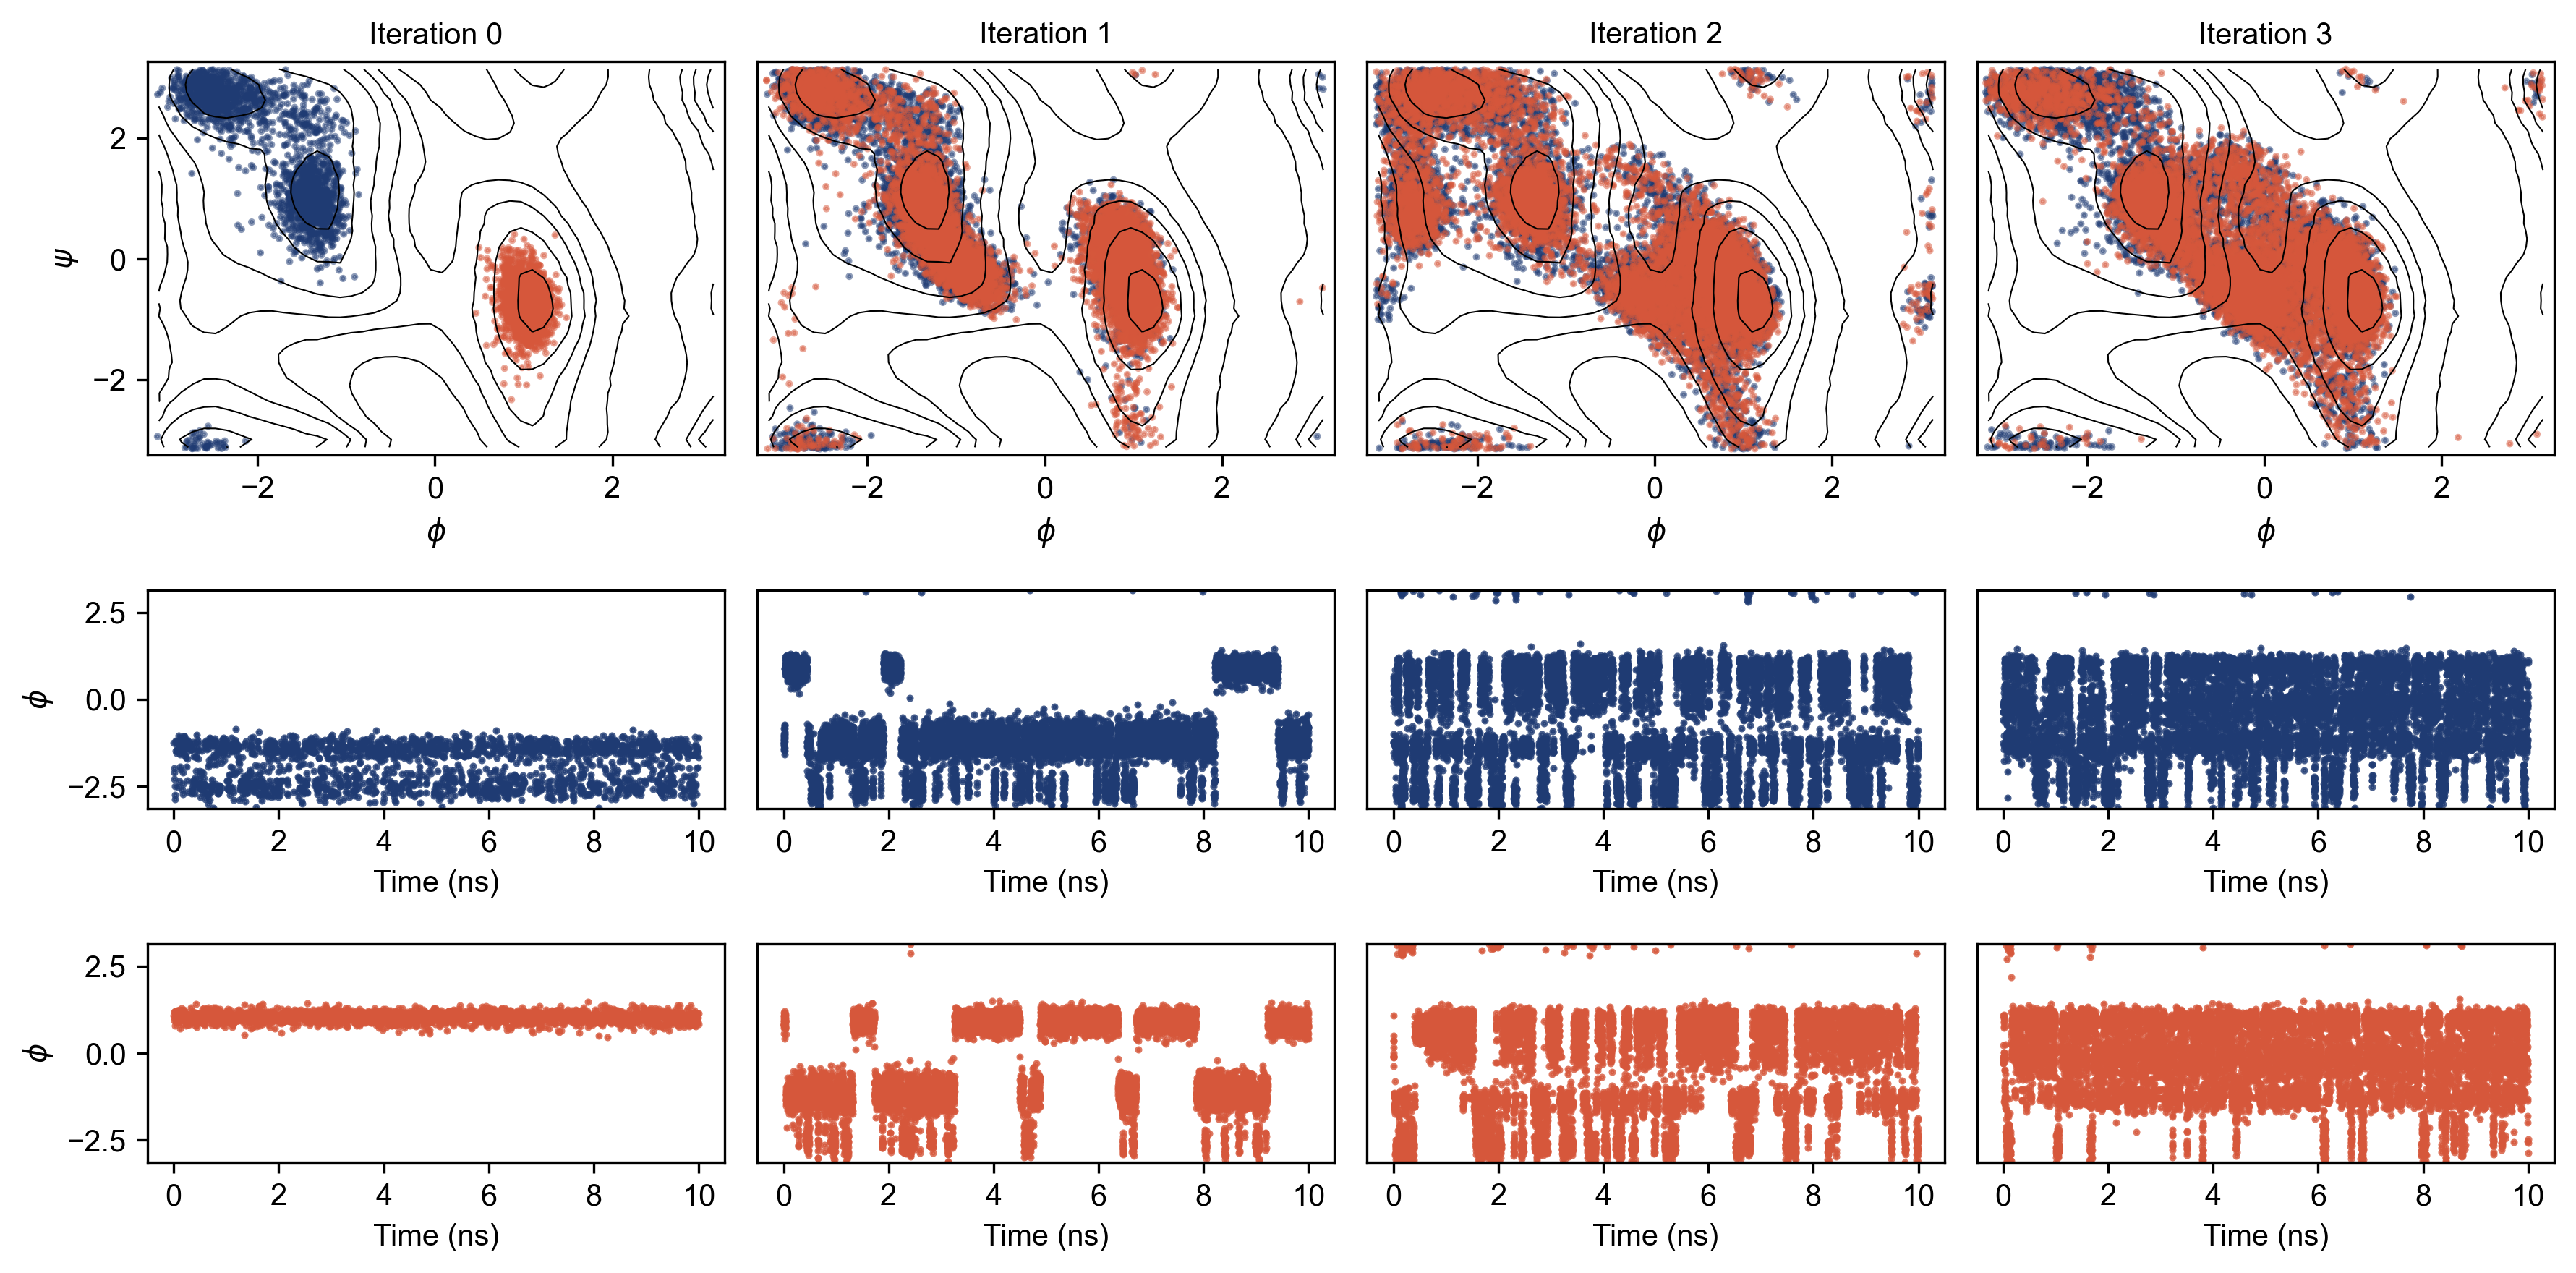
\includegraphics[width=1\linewidth]{Figures/SI/alanine/sampling.png}
        \caption{\textbf{Iterations sampling Alanine} Sampling at different iterations on the procedure on Alanine.
        Top row: Scatter plot of the sampled points in the $\phi\psi$ space. Points obtained starting the simulation in state A (left) are depicted in blue, and those sampled starting from state B (right) are in red..
        Middle row: Time series of the $\phi$ value from a trajectory started from state A.
        Bottom row: Time series of the $\phi$ value from a trajectory started from state B.}
        \label{sup_fig:alanine_sampling}
    \end{figure}

\clearpage
\section{Double path potential - Additional information}
    \subsection{Computational details}
        \paragraphtitle{Simulations details}
            The double path potential energy surface, $U(x, y)$, is defined as a function of the Cartesian coordinates $x$ and $y$ 
                \begin{equation}
                \begin{split}
                     U(x,y) = 10\bigg(2+\frac{4x^4}{3}-2y^2+y^4+\frac{10x^2(y^2-1)}{3}\bigg) \\
                     + 7\exp \bigg( -\frac{(x+0.7)^2 + (y-0.8)^2}{0.4^2}\bigg) \\
                     + \exp \bigg( -\frac{(x-1)^2 + (y+0.3)^2}{0.4^2}\bigg) \\ 
                     - 6\exp\bigg( -\frac{(x+1)^2 + (y+0.6)^2)}{0.4^2}\bigg) \\
                     -2.35906
                    \label{seq:double_path_formula}
                \end{split}
                \end{equation}
            
            The simulations of the diffusion of an ideal particle of mass 1 have been performed using Langevin dynamics based on the Bussi-Parrinello algorithm~\cite{bussi2007accurate} as implemented in the \texttt{ves\_md\_linearexpansion}~\cite{valsson2014variational} module of PLUMED.~\cite{tribello2014plumed, plumed2019promoting}
            The damping constant in the Langevin equation was set to  10/time-unit. 
            The time unit was defined arbitrarily and corresponds to 200 timesteps and natural units ($k_BT = 1$) were used in all the calculations.

        \paragraphtitle{Committor model training details}
            To model the committor function $q_\theta(\textbf{x})$ at each iteration, we used the x and y Cartesian coordinates of the diffusing particle as inputs of a neural network (NN) with architecture [2, 32, 32, 1] nodes/layer.
            For the optimization, we used the ADAM optimizer with an initial learning rate of $10^{-3}$ modulated by an exponential decay with multiplicative factor $\gamma=0.99999$. The training was performed for 5000 epochs in the first iteration and for $\sim$20000 epochs for the others. 
            The $\alpha$ hyperparameter in the loss function was set to 10.
            The number of iterations, the corresponding dataset size, and the $\lambda$ and the OPES \texttt{BARRIER} used in the biased simulations are summarized in Table~\ref{sup_tab:double_path_iterations} alongside the lowest value obtained for functional $K_m$ (e.q., the variational loss term $L_v$), which provides a quality and convergence measure, the simulation time $t_s$ and the output sampling time $t_o$. 
            \begin {table}[h!]
                \caption {\textbf{Summary double-path potential} Summary of the iterative procedure for double path potential.} \label{sup_tab:double_path_iterations}
                \vspace{-5mm}
                \begin{center}
                \begin{tabular}{ |c|c|c|c|c|c|c| } 
                 \hline
                 Iteration & Dataset size & $K_m$ [au] & OPES \texttt{BARRIER} [$k_BT$] & $\lambda$ & $t_s$ [au] & $t_o$ [au] \\ 
                 \hline
                    0   & 4000 &  35.77  & - & - & 2*5000000 & 500 \\
                    1   & 22000 &  1.38 & 20 & 1 & 2*5000000 & 500\\
                    2   & 40000 & 1.37  & 20 & 1 & 2*5000000 & 500 \\  
                 \hline
                \end{tabular}
                \end{center}
            \end {table}
    
    \vspace{-5mm}
    \subsection{Additional figures}
    \vspace{-5mm}
        \begin{figure}[h!]
            \centering
            
\includegraphics[width=0.8\linewidth]{Figures/SI/double_path/sampling.png}
            \caption{\textbf{Iterations sampling double-path} Sampling at different iterations of the procedure on the double path potential.
            Points obtained starting the simulation in state A (left) are depicted in blue, and those sampled starting from state B (right) are in red.
            The 0.5 value of the committor estimate at that iteration is provided as a black line.}
            \label{sup_fig:double_path_sampling}
        \end{figure}


\clearpage
\section{Chignolin - Additional information}
    \subsection{Computational details}
        \paragraphtitle{Simulations details}
            For the study of folding and unfolding of chignolin (CLN025 peptide sequence Tyr-Tyr-Asp-Pro-Glu-Thr-Gly-Thr-Trp-Tyr) in explicit solvent, we performed our simulations using GROMACS v2021.5~\cite{abraham2015gromacs} patched with PLUMED,~\cite{tribello2014plumed, plumed2019promoting} the CHARMM22$^*$~\cite{piana2011robust} force field, and the solvent has been modeled by the CHARMM TIP3P~\cite{mackerell1998tip} force field, sharing the same setup used for long unbiased simulations on this system~\cite{lindorff2011fast} to have a direct comparison with those results. 
            For the same reason, we kept the simulation condition consistent with that work.
            All simulations were performed with an integration time step of 2 fs and sampling NVT ensemble at 340K. Asp, Glu residues, as well as the N- and C-terminal amino acids are simulated in their charged states. The simulation box contains 1,907 water molecules, together with two sodium ions that neutralize the system. The linear constraint solver algorithm is applied to every bond involving H atoms, and electrostatic interactions are computed via the particle mesh Ewald scheme, with a cutoff of 1 nm for all nonbonded interactions.

        \paragraphtitle{Committor model training details}
            To model the committor function $q_\theta(\textbf{x})$ at each iteration, we used the 210 distances suggested by Ref.~\citenum{bonati2021deep} as inputs of a neural network (NN) with architecture  [210, 64, 32, 1] nodes/layer.
            For the optimization, we used the ADAM optimizer with an initial learning rate of $10^{-3}$ modulated by an exponential decay with multiplicative factor $\gamma=0.99995$. 
            The training was performed for $\sim$30000 epochs. The $\alpha$ hyperparameter in the loss function was set to 1.
            The number of iterations, the corresponding dataset size, and the $\lambda$ and the OPES \texttt{BARRIER} used in the biased simulations are summarized in Table~\ref{sup_tab:chignolin_iterations} alongside the lowest value obtained for the functional $K_m$, which provides a quality and convergence measure, the simulation time $t_s$ and the output sampling time $t_o$.
            \begin {table}[h!]
                \caption {\textbf{Summary Chignolin} Summary of the iterative procedure for chignolin.} \label{sup_tab:chignolin_iterations}
                %\vspace{-5mm}
                \begin{center}
                \begin{tabular}{ |c|c|c|c|c|c|c| } 
                 \hline
                 Iteration & Dataset size & $K_m$ [au] & OPES \texttt{BARRIER} [kJ/mol] & $\lambda$ & $t_s$ [ns] & $t_o$ [ps] \\ 
                 \hline
                    0   & 20000 &  27.36  & -& -     & 2*100 & 10\\
                    1   & 220000 &  4.43 & 20& 0.3  & 4*250 & 5\\
                    2   & 220000 &  3.64 & 20& 0.3  & 4*250 & 5\\
                    3   & 220000 &  3.79 & 20& 0.3  & 4*250 & 5\\
                    4   & 220000 &  2.32 & 20& 0.3  & 4*250 & 5\\
                    5   & 220000 &  2.17 & 20& 0.3  & 4*250 & 5\\   
                 \hline
                \end{tabular}
                \end{center}
            \end {table}

    \subsection{Additional results}
    \paragraphtitle{Comparison between different descriptor sets}
        In Ref.~\citenum{kang2024computing}, we trained the committor model using as inputs the 45 distances between $\alpha$-C atoms, whereas here, we used the same set of 210 distances identified in Ref.~\citenum{bonati2021deep}.
        To compare the two descriptor sets, we optimized the committor model on the same dataset using the two sets, obtaining a $K_m$ value of 2.17 for the 210 distances and 18.5 for the 45 distances.
        This result clearly shows how the greater variational flexibility introduced by side-chain information allows for capturing more features of the folding process.

    \paragraphtitle{LASSO Analysis}
        To analyze the relevance of the input feature in the trained model, we applied the LASSO regression analysis~\cite{novelli2022lasso} on several bins along $z$ values. 
        The results of this analysis are summarized in Tab.~\ref{sup_tab:chignolin_lasso}, where the 5 most important descriptors for each bin are reported alongside the corresponding bin range.
        
            \begin {table}[h!]
                \caption {\textbf{LASSO summary Chignolin} Summary of LASSO analysis for chignolin. The atoms involved in the distances used as descriptors are indicated according to the indexes used in PLUMED (upper table) and their names from the PDB (lower table).} \label{sup_tab:chignolin_lasso}
                %\vspace{-5mm}
                \begin{center}
                \begin{tabular}{ |c|c| } 
                 \hline
                 z range & Top 5 ranking distances \\ 
                 \hline
                    $-5.5\sim -4.3$  & $d_{102-139},d_{107-139},d_{102-141},d_{109-131},d_{78-141}$\\
                    $-4.3\sim -3.2$ & $d_{102-139},d_{102-141},d_{107-139},d_{78-141},d_{109-131}$\\
                    $-3.2\sim -2.0$  &$d_{36-102},d_{23-145},d_{36-70},d_{7-145},d_{45-147}$\\
                    $-2.0\sim -0.8$  &$d_{22-164},d_{37-69},d_{23-164},d_{37-109},d_{43-120}$\\
                    $-0.8\sim 0.3$ &   $d_{22-164},d_{23-164},d_{36-105},d_{23-145},d_{37-69}$\\
                    $0.3\sim 1.5$  &  $d_{23-145},d_{43-120},d_{23-106},d_{36-144},d_{44-152}$\\
                    $1.5\sim 2.7$ &$d_{43-120},d_{44-152},d_{23-145},d_{37-109},d_{37-66}$\\
                    $2.7\sim 3.8$&  $d_{52-86},d_{63-105},d_{31-100},d_{41-141},d_{56-105}$\\
                    $3.8\sim 5.0$ &   $d_{43-120},d_{31-115},d_{52-86},d_{49-111},d_{41-144}$\\
                    $5.0\sim 6.1$& $d_{34-128},d_{52-94},d_{52-83},d_{1-152},d_{11-165}$\\
                 \hline
                \end{tabular}
                
                \vspace{8mm}
                
                \begin{tabular}{ |c|c| } 
                 \hline
                 z range & Top 5 ranking distances \\ 
                 \hline
                    $-5.5\sim -4.3$& Gly7-CA:Trp9-CZ2, Thr8-N:Trp9-CZ2,  Gly7-CA:Trp9-CH2, Thr8-CA:Trp9-NE1,  Glu5-CG:Trp9-CH2\\
                    $-4.3\sim -3.2$& Gly7-CA:Trp9-CZ2, Gly7-CA:Trp9-CH2, Thr8-N:Trp9-CZ2,  Glu5-CG:Trp9-CH2,  Thr8-CA:Trp9-NE1\\
                    $-3.2\sim -2.0$& Tyr2-CZ:Gly7-CA,  Tyr1-O:Tyr10-N,   Tyr2-CZ:Pro4-O,   Tyr1-CB:Tyr10-N,   Asp3-N:Tyr10-CA\\
                    $-2.0\sim -0.8$& Tyr1-C:Tyr10-C,   Tyr2-OH:Pro4-C,   Tyr1-O:Tyr10-C,   Tyr2-OH:Thr8-CA,   Tyr2-C:Thr8-O\\
                    $-0.8\sim 0.3$ & Tyr1-C:Tyr10-C,   Tyr1-O:Tyr10-C,   Tyr2-CZ:Gly7-C,   Tyr1-O:Tyr10-N,    Tyr2-OH:Pro4-C\\
                    $0.3\sim 1.5$  & Tyr1-O:Tyr10-N,   Tyr2-C:Thr8-O,    Tyr1-O:Gly7-O,    Tyr2-CZ:Trp9-O,    Tyr2-O:Tyr10-CG\\
                    $1.5\sim 2.7$  & Tyr2-C:Thr8-O,    Tyr2-O:Tyr10-CG,  Tyr1-O:Tyr10-N,   Tyr2-OH:Thr8-CA,   Tyr2-OH:Pro4-CG\\
                    $2.7\sim 3.8$  & Asp3-CG:Thr6-N,   Pro4-CB:Gly7-C,   Tyr2-CG:Gly7-N,   Tyr2-CE2:Trp9-CH2, Asp3-O:Gly7-C\\
                    $3.8\sim 5.0$  & Tyr2-C:Thr8-O,    Tyr2-CG:Thr8-CG2, Asp3-CG:Thr6-N,   Asp3-CB:Thr8-CB,   Tyr2-CE2:Trp9-O\\
                    $5.0\sim 6.1$  & Tyr2-CE1:Trp9-CG, Asp3-CG:Thr6-CG2, Asp3-CG:Glu5-OE2, Tyr1-N:Tyr10-CG,   Tyr1-CD1:Tyr10-HE2\\
                 \hline
                \end{tabular}
                \end{center}
            \end {table}

\newpage
    \paragraphtitle{Free energy surfaces}
        \begin{figure}[h!]
            \centering
            
\includegraphics[width=0.8\linewidth]{Figures/SI/chignolin/fes_z_q.png}
            \caption{\textbf{Free energy surface Chignolin} Free energy estimates for Chignolin projected along $z$ and $q$ obtained averaging on 6 independent simulations: 3 started from the folded state and 3 from the unfolded one. 
            The average value and the relative standard deviation are reported as a solid line and a shaded region, respectively.}
            \label{sup_fig:chignolin_fes_z_q}
        \end{figure}

\clearpage
\section{Calixarene - Additional information}
    \subsection{Computational details}
        \paragraphtitle{Simulations details}
            We performed the simulations with GROMACS~\cite{abraham2015gromacs} v2021.5 in combination with the PLUMED~\cite{tribello2014plumed, plumed2019promoting} plugin. We use the GAFF~\cite{wang2004development} force field with RESP~\cite{bayly1993well} charges and the TIP3P~\cite{jorgensen1983comparison} water model. 
            We set the timestep to 2 fs and the temperature at 300 K via a velocity rescale thermostat~\cite{bussi2007velocity} with a time constant of 0.1 ps.
            The simulation box is cubic with a side of 40.27 $\si{\angstrom}$ and it contains 2100 water molecules in solution together with the host OAMe and the chosen guest molecule. 
            Sodium ions are included to counterbalance excess charges. 
            At every simulation step, the coordinates are aligned so that the vertical axis of the box coincides with the binding axis $h$, and the simulation box is centered on the virtual atom V1.

        \paragraphtitle{The funnel restraint}
        \label{sup_sec:funnel_restraint}
            In our simulations, we used a funnel restraint~\cite{limongelli2013funnel} equivalent to the one previously employed by Refs.\citenum{rizzi2021role,bhakat2017resolving,perez2019local} on the same system.
            Here, we summarize the details of such a restraint, while more details can be found in the original works.
            The funnel limits the space available to the ligand in the unbound state U by confining it to a cylindrical volume above the binding site. 
            As the ligand approaches the binding site, the funnel restraint becomes wider so that its presence does not affect the binding process itself. 
            Having aligned with PLUMED the system to a reference configuration where the binding axis is found along the vertical axis, we define $h$ as the projection on the binding axis of the center of the carbon atoms of each ligand and $r$ as its radial component.
            When $h>10 \si{\angstrom}$, the funnel surface is a cylinder with radius $R_{cyl} = 2 \si{\angstrom}$ with its axis along the vertical direction. 
            When $h<10 \si{\angstrom}$, the funnel opens into an umbrella-like shape with a 45 degree angle whose surface is defined by $r=12-h$.
            The force that, for a displacement x, pushes the ligand away from the funnel’s surface is harmonic $-k_Fx$ with $kF=20 $ kJ/mol $\si{\angstrom}^{-2}$. 
            A further harmonic restraint is applied on $h$  to prevent the ligand from getting too far from the host, reaching the upper boundary of the simulation box. 
            The corresponding force is $-k_U(h-18)$ for $h > 18\si{\angstrom}$ and $k_U=40 $ kJ/mol $\si{\angstrom}^{-2}$.

            During training, we set boundaries further to state U so that the labeled configurations used to impose the boundary conditions will not influence the committor training in the subsequent iterative simulations.
            We apply the funnel restraint described above and two additional harmonic restraints $-k_U(h-20)$ for $h > 20 \si{\angstrom}$ and $-k_U(h-18)$ for $h < 18 \si{\angstrom}$, with $k_U = 20$ kJ/mol.
        
            Because of the funnel presence, the free energy difference between the bound and the true unbound state that we extract from enhanced sampling simulations needs a correction that can be calculated as:
                \begin{equation}
                    \Delta G = -\frac{1}{\beta} \log \left( C_0 \pi R_{\text{cyl}}^2 \int_B dh \exp\left[-\beta \left(W(h) - W_U\right)\right] \right)
                \end{equation}
            where $\beta$ = 1/($k_B$T), $C_0$ = 1/1660 $\si{\angstrom}^{-3}$ is the standard concentration, $h$ is the coordinate along the funnel’s axis, $W(h)$ is the free energy along the funnel axis and $W_U$ its reference value in state U. 
            More precisely, we define $W_U$ as the average free energy value in the interval 1.6  $\si{\angstrom}$ < $h$ < 1.8  $\si{\angstrom}$.
            The integral is computed over the state B region that we define as 0.3  $\si{\angstrom}$ < $h$ < 0.8  $\si{\angstrom}$.

        \paragraphtitle{Committor model training details}
            To model the committor function $q_\theta(\textbf{x})$ at each iteration, we used the same water coordination numbers used in Ref.~\citenum{rizzi2021role}, 8 with respect to 2.5\AA-spaced virtual atoms (V) along the binding axis and 4 with respect to 4 atoms on the ligand molecule (M) (2 on the ring (1 and 2), 2 on the terminal atoms (3 and 4)), and a set of distances between the same 4 ligand atoms and the binding pocket, instead of the $h$ projection only, as inputs of a neural network (NN) with architecture [16, 32, 32, 1] nodes/layer.
            For the optimization, we used the ADAM optimizer with an initial learning rate of $10^{-3}$ modulated by an exponential decay with multiplicative factor $\gamma=0.99995$.
            The training was performed for $\sim$30000 epochs. 
            The $\alpha$ hyperparameter in the loss function was set to 1.
            In the loss function, we assigned to the virtual points along the binding axis used for the computation of water coordination numbers an \emph{infinite} mass, that is, $10^6$.
            The number of iterations, the corresponding dataset size, and the $\lambda$ and the OPES \texttt{BARRIER} used in the biased simulations are summarized in Table~\ref{sup_tab:calixarene_iteration} alongside the lowest value obtained for the functional $K_m$, which provides a quality and convergence measure, the simulation time $t_s$ and the output sampling time $t_o$.

            \begin {table}[h!]
                \caption {\textbf{Summary calixarene} Summary of the iterative procedure for calixarene.} \label{sup_tab:calixarene_iteration}
                %\vspace{-5mm}
                \begin{center}
                \begin{tabular}{ |c|c|c|c|c|c|c| } 
                 \hline
                 Iteration & Dataset size & $K_m$ [au] & OPES \texttt{BARRIER} [kJ/mol] & $\lambda$ & $t_s$ [ns] & $t_o$ [ps] \\ 
                 \hline
                    0   & 2000 &  27400  & -& -     & 2*10 & 10\\
                    1   & 22000 &  137 & 50& 0.6  & 2*100 & 10\\
                    2   & 22000 &  333 & 50& 0.6  & 2*100 & 10\\
                    3   & 22000 &  242 & 50& 0.6  & 2*100 & 10\\
                    4   & 22000 &  5.16 & 50& 0.6  & 2*100 & 10\\
                    5   & 22000 &  4.56 & 50& 0.6  & 2*100 & 10\\
                 \hline
                \end{tabular}
                \end{center}
            \end {table}

    \newpage
    \subsection{Additional results}
    \paragraphtitle{Feature relevance analysis}
        \begin{figure}[h!]
            \centering
            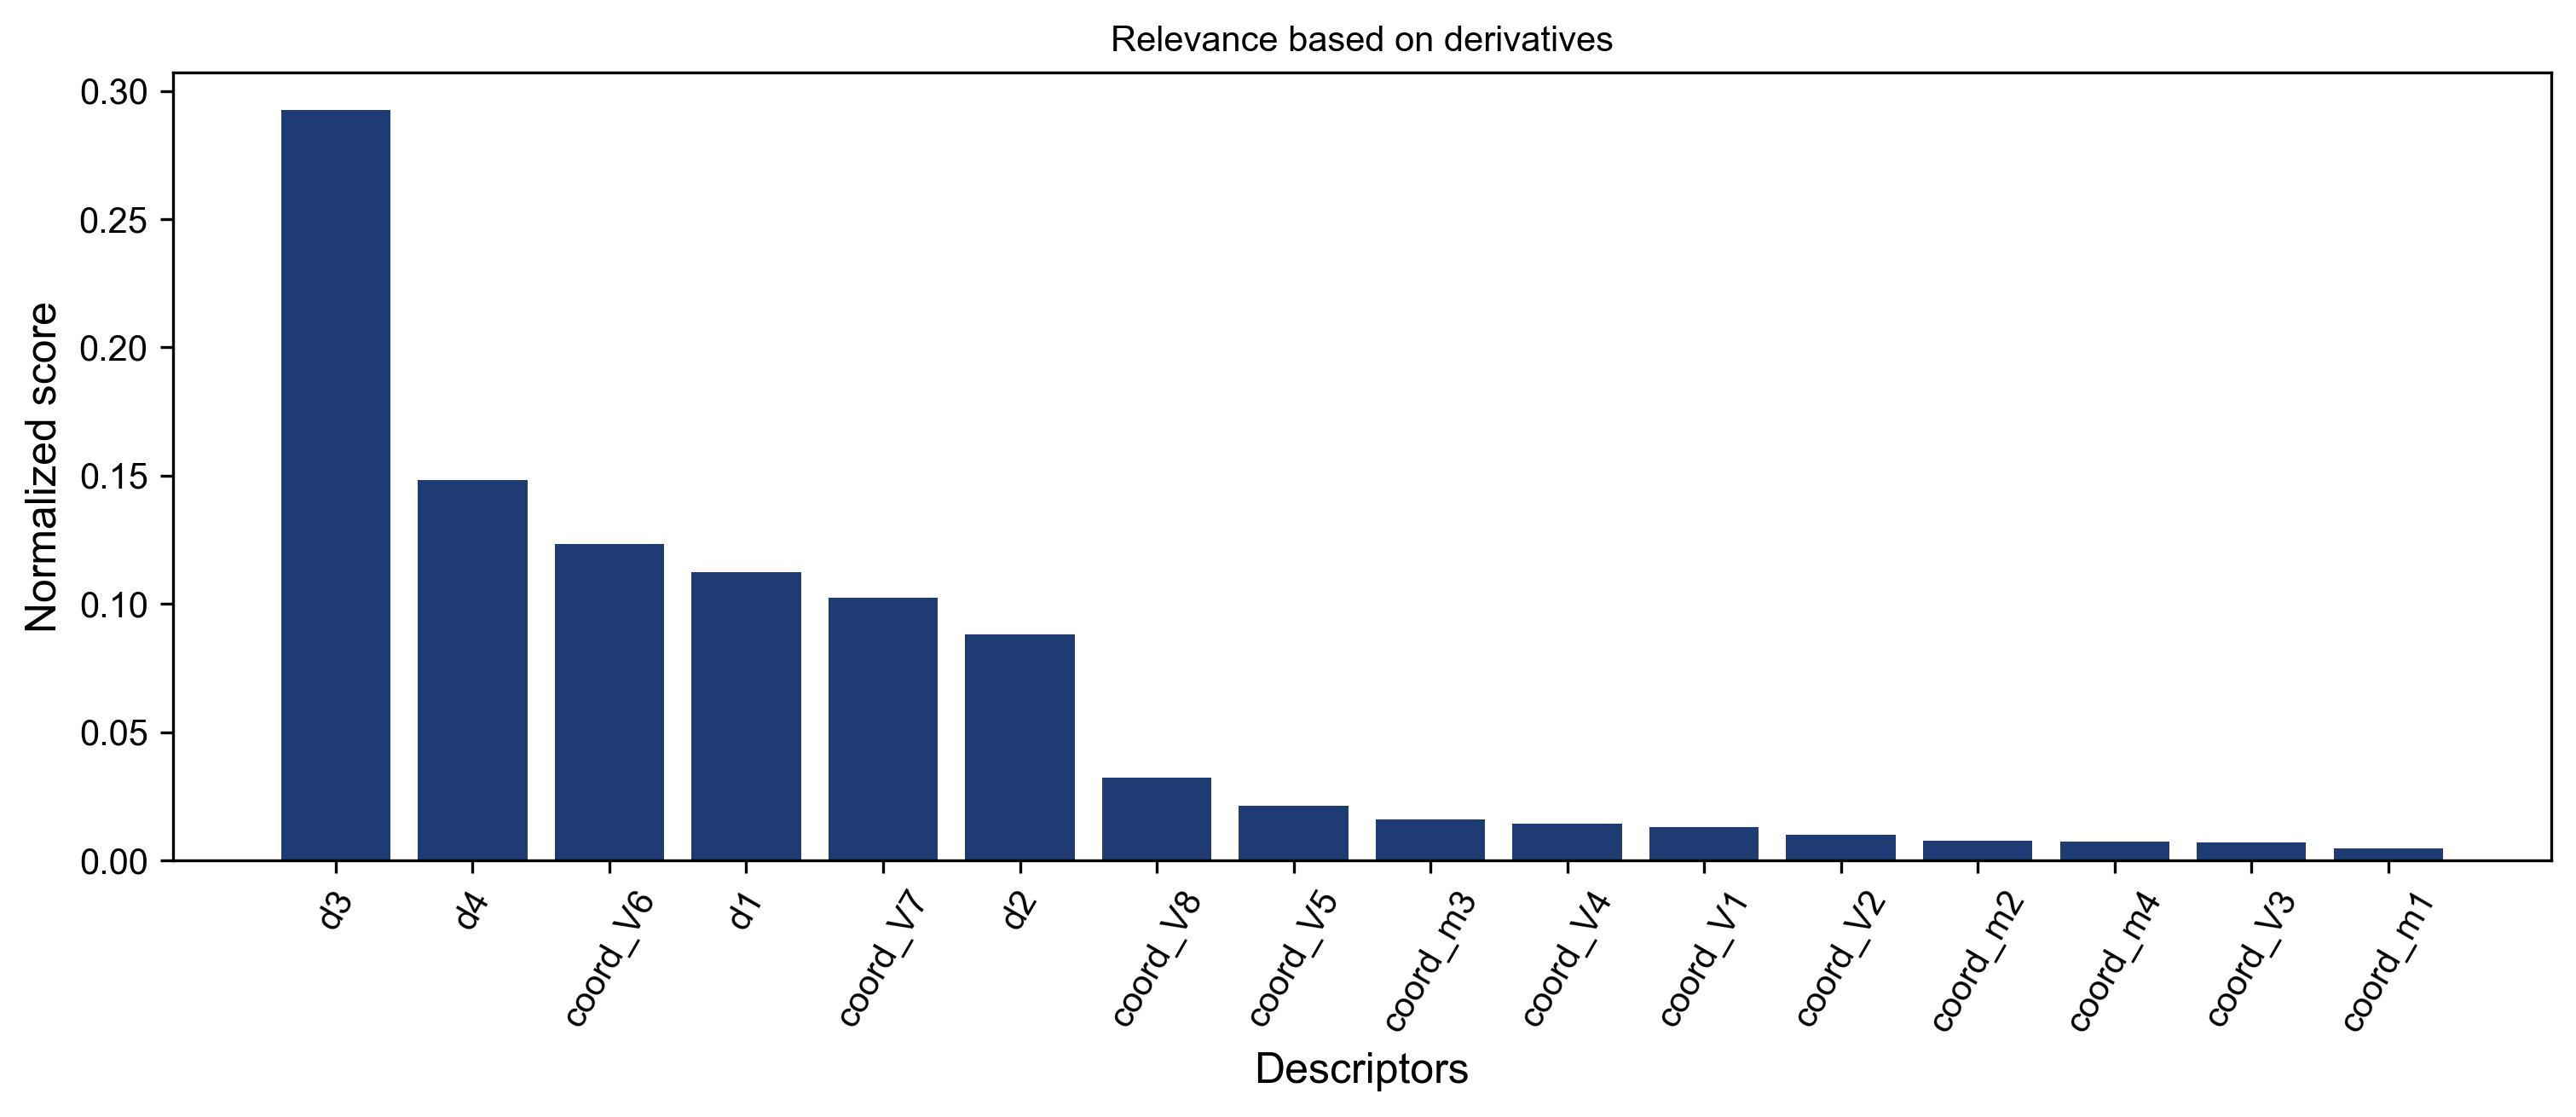
\includegraphics[width=0.8\linewidth]{Figures/SI/calixarene/calixarene_ranking.png}
            \caption{\textbf{Feature relevance calixarene} Descriptors ranking for the committor model of calixarene trained using the descriptors listed in the computational details.}
            \label{sup_fig:calixarene_feature_relevance}
        \end{figure}
        
    \paragraphtitle{Free energy surfaces}
        \begin{figure}[h!]
            \centering
            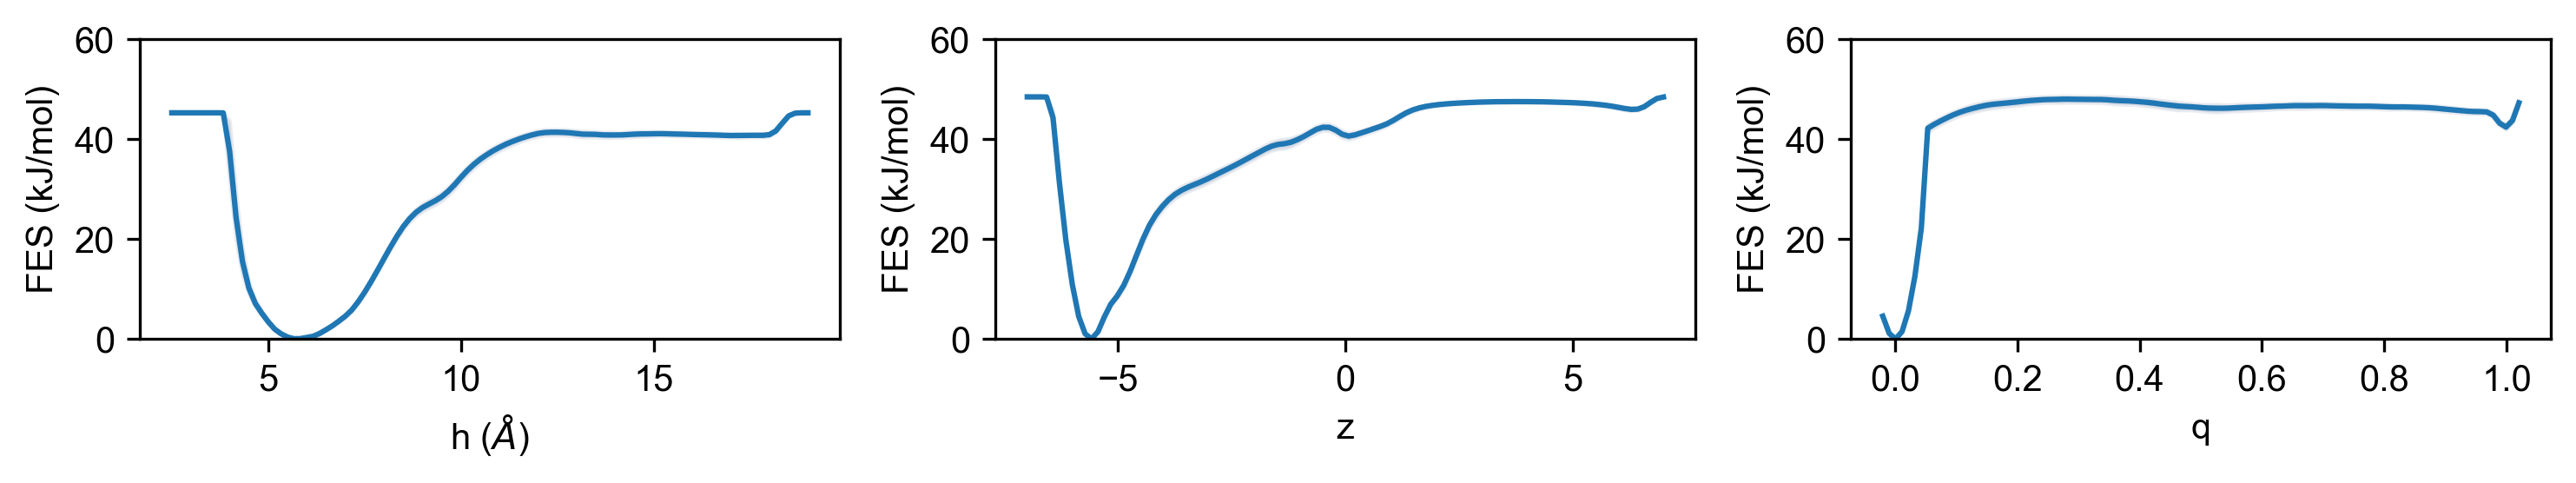
\includegraphics[width=1\linewidth]{Figures/SI/calixarene/fes_z_q.png}
            \caption{\textbf{1D free energy surface calixarene} Free energy estimates for calixarene projected along the projection of the ligand molecule on the binding axis $h$, $z$ and $q$.}
            \label{sup_fig:Calixarene_fes_z_q}
        \end{figure}

        \begin{figure}[h!]
            \centering
            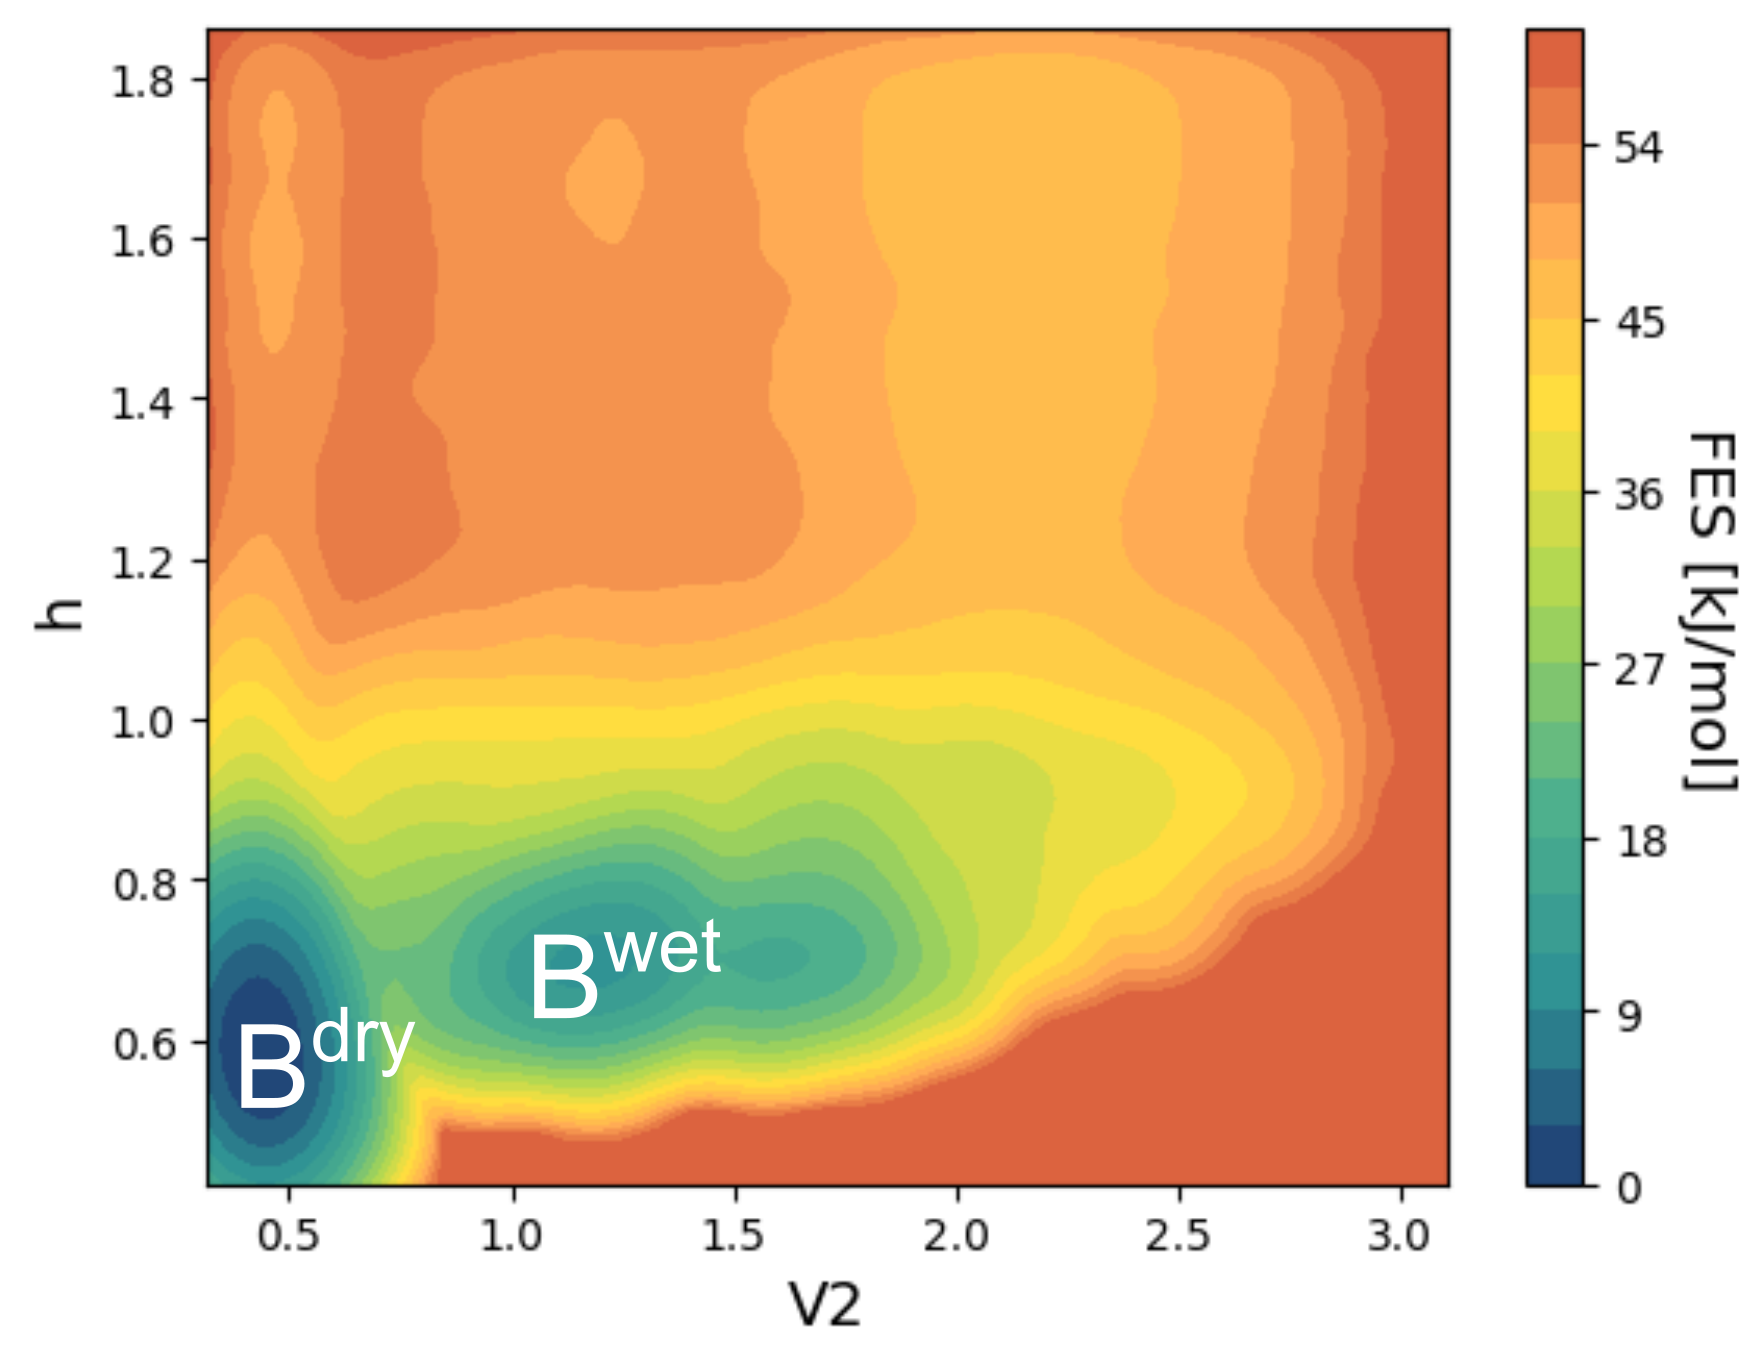
\includegraphics[width=0.5\linewidth]{Figures/SI/calixarene/2DFES.png}
            \caption{\textbf{2D free energy surface calixarene} Two-dimensional free energy surface for calixarene projected in the plane defined by the water coordination number of a virtual point inside the binding cavity (V2) and the projection of the ligand molecule on the binding axis (h). }
            \label{sup_fig:Calixarene_2DFES}
        \end{figure}

    \newpage
    \paragraphtitle{Kolmogorov Ensemble}

        \begin{figure}[h!]
            \centering
            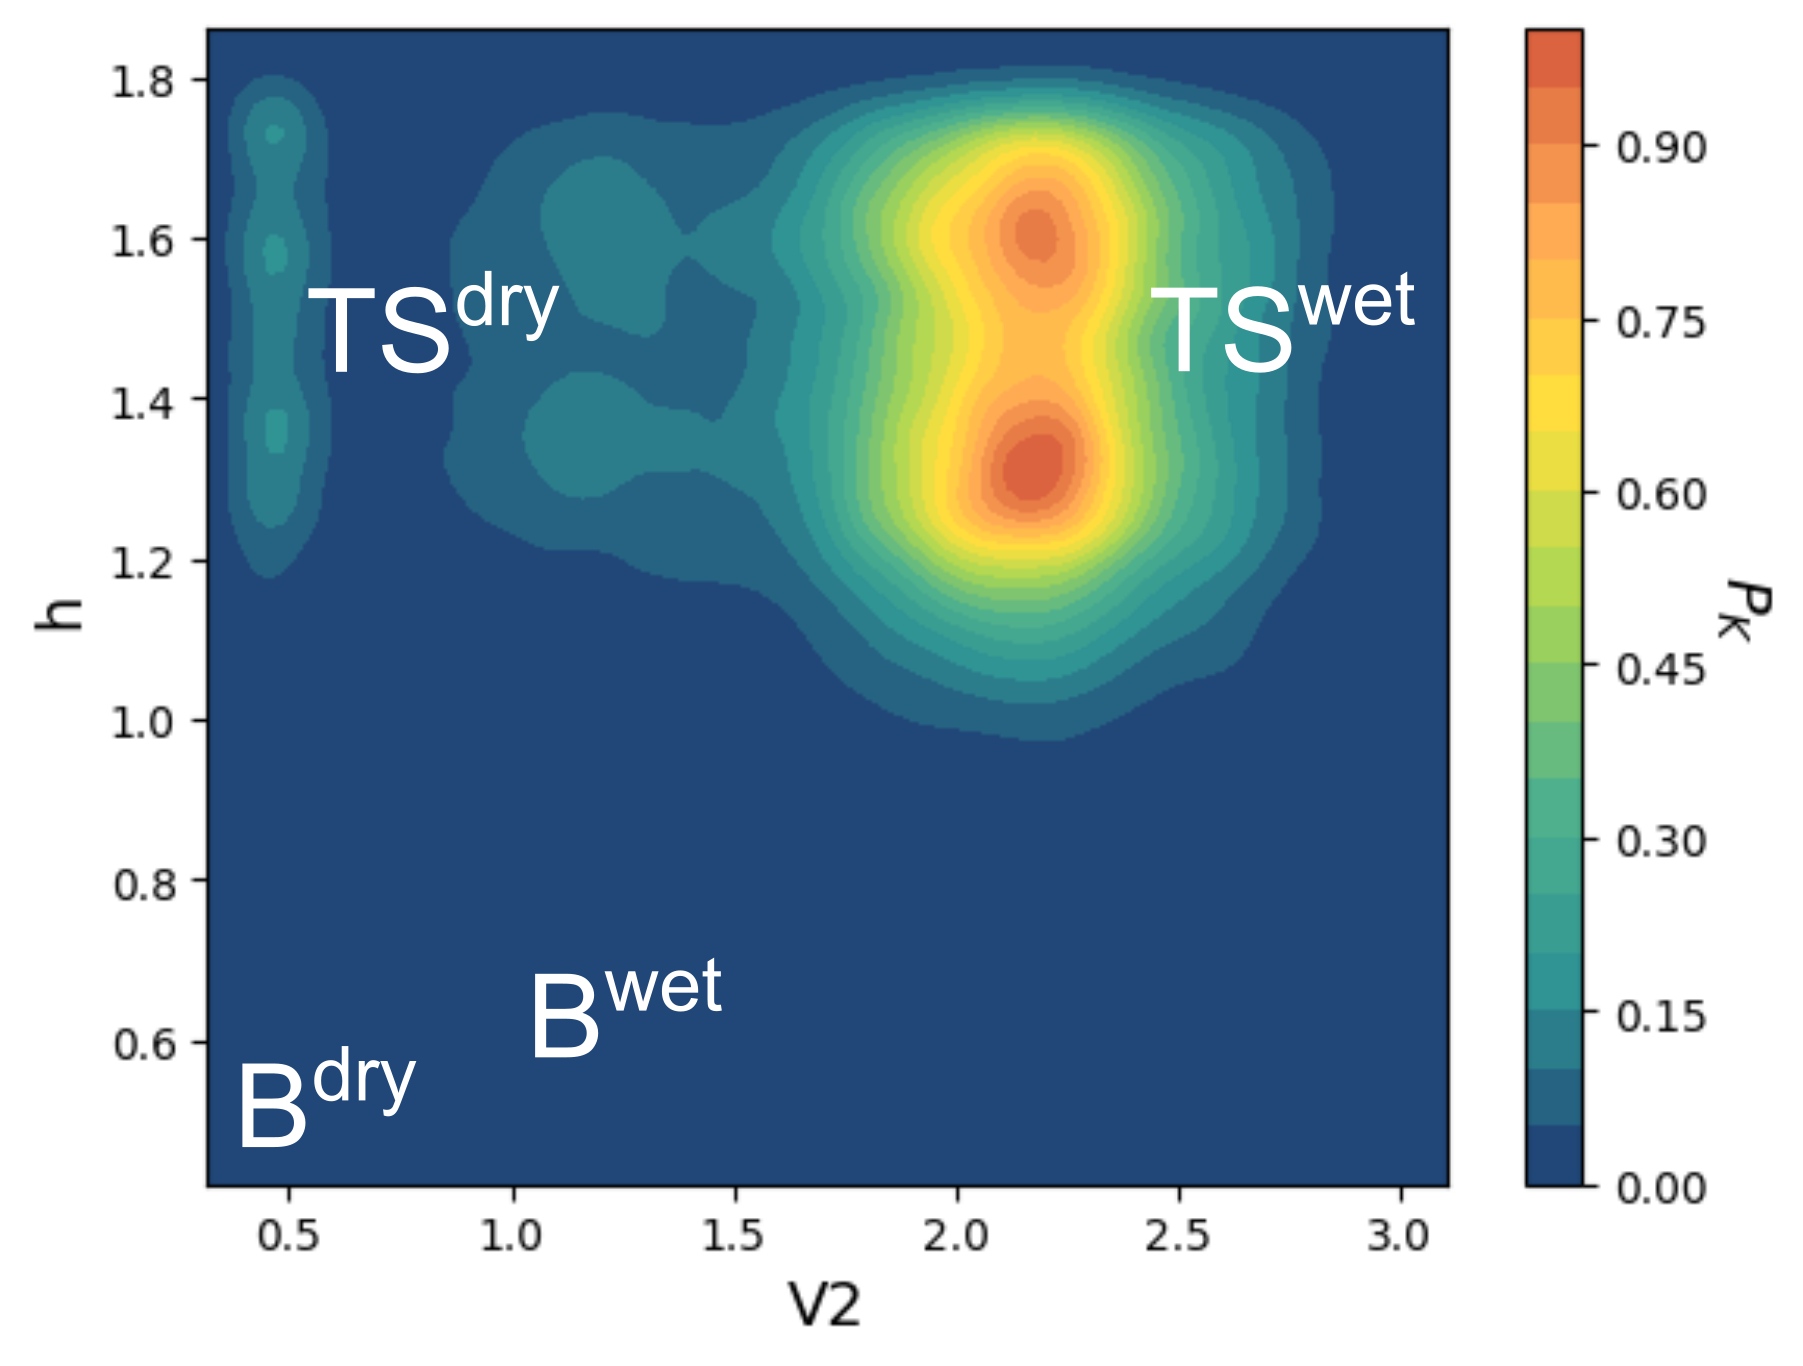
\includegraphics[width=0.5\linewidth]{Figures/SI/calixarene/KolmogorovDistribution.png}
            \caption{\textbf{Kolomogorov distribution calixarene} Two-dimensional Kolmogorov probability $p_K$ projection for calixarene projected in the plane defined by the water coordination number of a virtual point inside the binding cavity (V2) and the projection of the ligand molecule on the binding axis (h). }
            \label{sup_fig:Calixarene_2D_K}
        \end{figure}


        % \begin{figure}[h!]
        %     \centering
        %     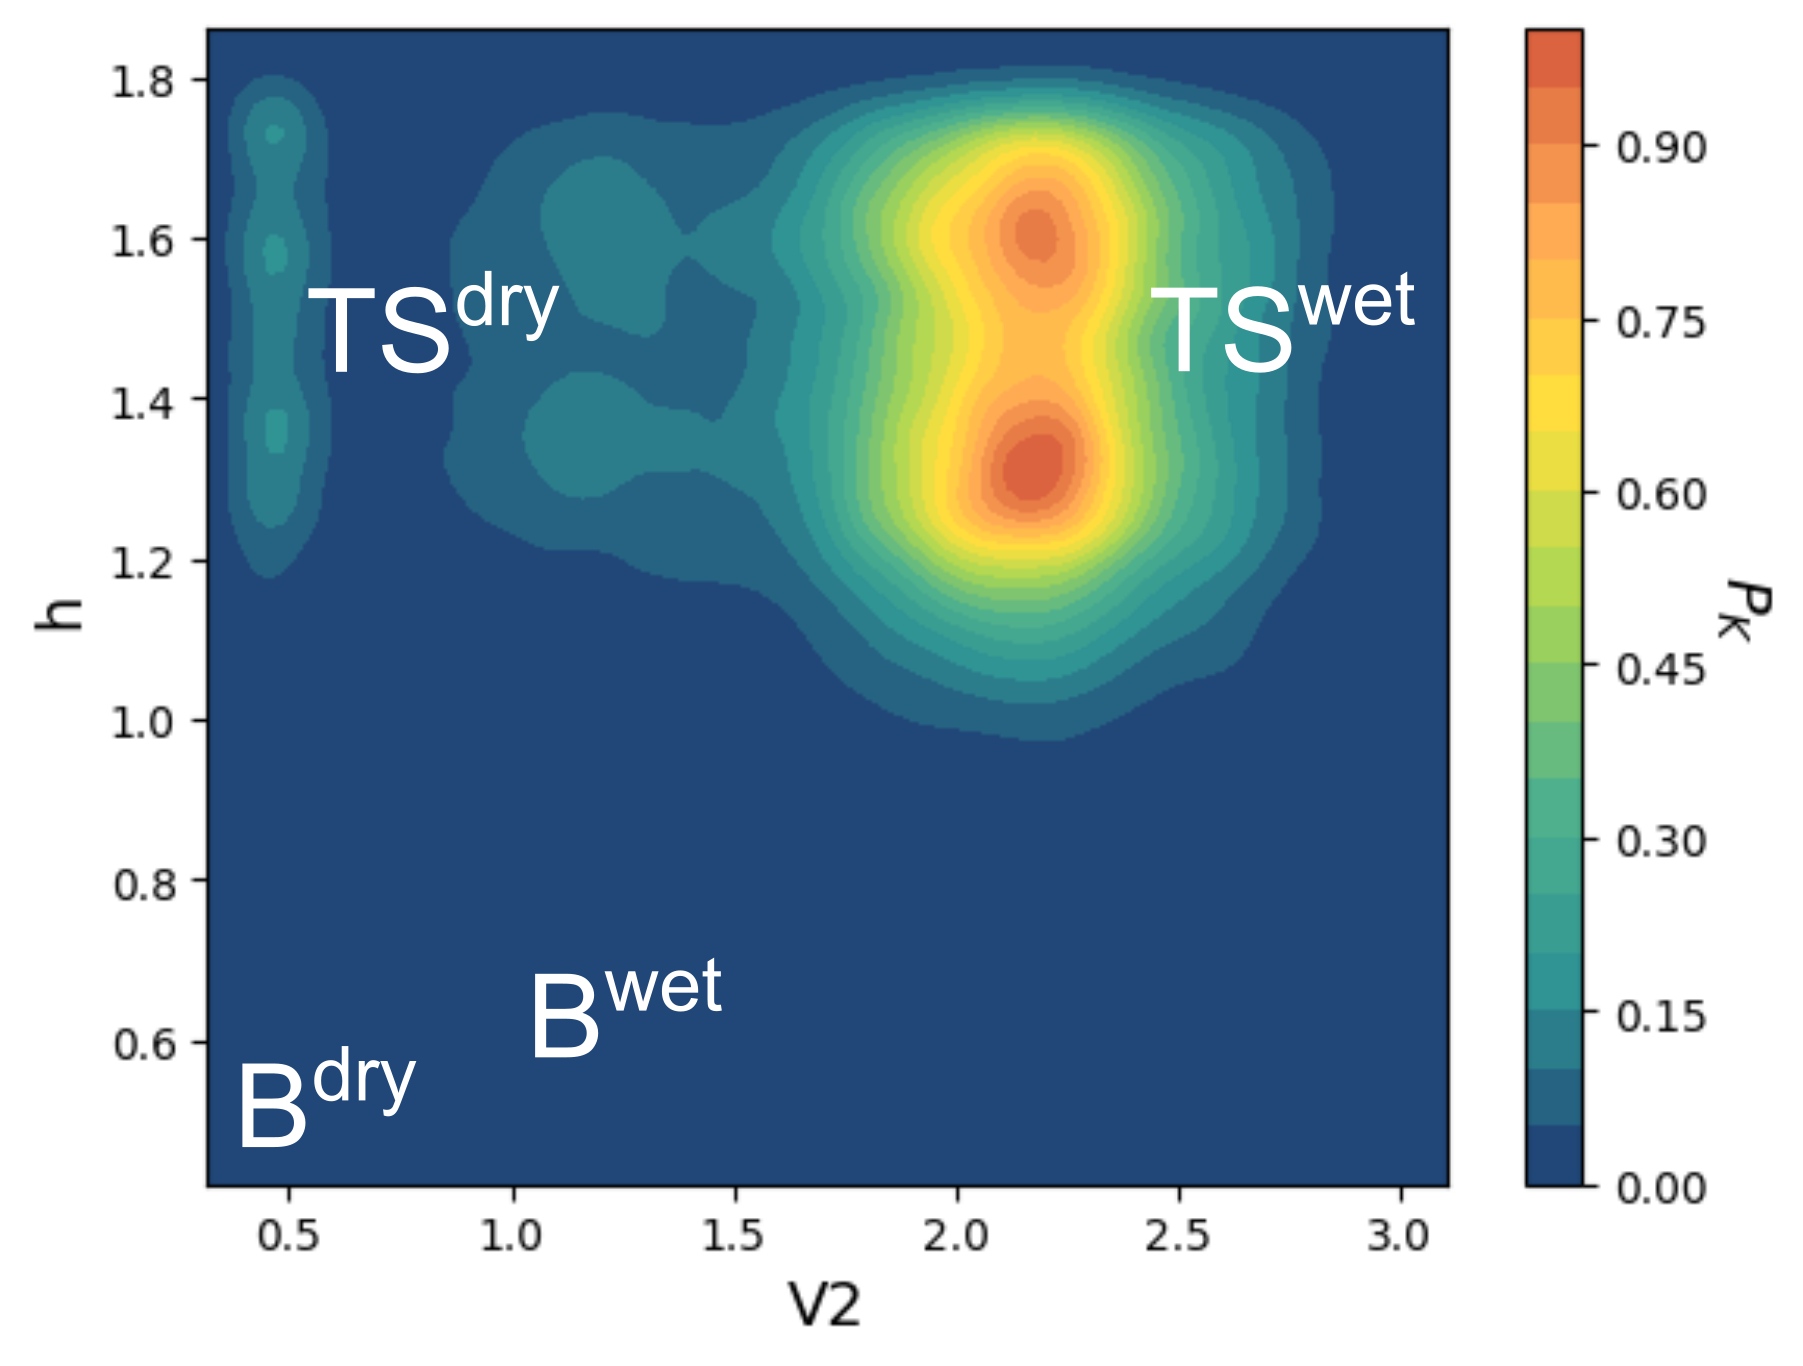
\includegraphics[width=0.6\linewidth]{Figures/SI/calixarene/KolmogorovDistribution.png}
        %     \caption{DeltaF for Calixarene}
        %     \label{sup_fig:Calixarene_Kolmogorov}
        % \end{figure}

    
        % \begin{figure}[h!]
        %     \centering
        %     \includegraphics[width=0.8\linewidth]{Figures/main/Calixarene_DeltaF.png}
        %     \caption{DeltaF for Calixarene}
        %     \label{sup_fig:Calixarene_deltaF}
        % \end{figure}